% Provenance (never printed): see sources/outline_sources.md (Year 3:
% geophysical fluid dynamics: rotating-frame equations, Rossby number,
% hydrostatic and geostrophic balance, thermal wind, buoyancy frequency).
% Brief: sources/book5/BRIEFS.md, ch. 19. Curves from
% figdata/bachelor-3/inertial_oscillation.py, thermal_wind.py and
% buoyancy_frequency.py. Exercise and problem values in the Book 5 scratch
% calculator calc/ch19.py. The Steppe of Orrin, its lake, its stations and
% its winds are invented.
\chapter{Dinamika Fluida Geofisika}\label{ch:b3:gfd-foundations}

Aduk secangkir teh dan pusarannya hilang dalam semenit; daun teh berkumpul di
tengah dasar cangkir, dan tidak ada yang terjadi lagi. Lautan dan atmosfer
juga teraduk oleh Matahari dan angin, tetapi di planet yang berotasi dan dalam
lapisan dengan massa jenis berbeda. Rotasi dan stratifikasi membuat keduanya tunduk
pada aturan yang tak pernah tampak di cangkir teh: angin bertiup sejajar isobar,
bukan melintasinya, kolom fluida menolak untuk miring, dan angin di troposfer atas
ditentukan oleh suhu di bawahnya. Bab ini menyusun persamaan untuk
aliran besar, lambat, dan tipis ini, serta beberapa bilangan yang
menentukan suku mana yang penting.

\begin{recall}
Gaya Coriolis dan gaya sentrifugal dalam kerangka berputar, persamaan Navier--Stokes
dan persamaan kontinuitas, viskositas, bilangan Reynolds, dan relasi hidrostatik
dibahas di buku fisika. Parameter Coriolis $f = 2\Omega
\sin\varphi$, gaya gradien tekanan, keseimbangan geostrofik,
angin geostrofik dan \omterm{def:b3:gfd-foundations:gradient}{angin gradien}, serta arus jet dibahas di volume Tahun~1
pada bab tentang sirkulasi umum atmosfer;
lapisan Ekman pada bab tentang sirkulasi samudra; suhu potensial,
stabilitas statis, dan osilasi parsel udara yang terangkat pada
bab tentang struktur atmosfer dan samudra.
\end{recall}

\section{Persamaan dalam kerangka berputar}\label{sec:b3:gfd-foundations:equations}

Dalam kerangka yang berputar bersama Bumi dengan kecepatan sudut
$\vec\Omega$, sebuah parsel fluida berkecepatan $\vec u$ mematuhi
\[
\frac{\mathrm D\vec u}{\mathrm Dt} + 2\vec\Omega\times\vec u =
-\frac{1}{\rho}\nabla p + \vec g + \nu\nabla^2\vec u ,
\qquad
\frac{\partial\rho}{\partial t} + \nabla\cdot(\rho\vec u) = 0 ,
\]
dengan $\mathrm D/\mathrm Dt = \partial/\partial t + \vec u\cdot\nabla$ adalah
turunan yang mengikuti parsel dan $\nu$ viskositas kinematik. Gaya
sentrifugal telah digabungkan ke dalam gravitasi: jumlahnya $\vec g$ adalah
gravitasi efektif, tegak lurus terhadap permukaan \omterm{def:b3:gravity-geodesy:geopotential}{geopotensial} tetap, dan
vertikal didefinisikan olehnya. Hanya suku Coriolis, $-2\vec\Omega\times
\vec u$, yang tersisa dari rotasi, dan suku ini tidak melakukan usaha: ia memutar
parsel tanpa mengubah lajunya. Bumi berputar dengan $\Omega =
\qty{7.292115e-5}{rad/s}$, sekali per hari sideris sebesar \qty{23.9345}{h}.
% ledger: geod5:grs80-defining, earth:Trot

Untuk gerak pada jarak yang jauh lebih kecil daripada jari-jari Bumi $a$, sebuah
kerangka Kartesius lokal sudah memadai: $x$ ke timur, $y$ ke utara, $z$ ke atas,
pada lintang $\varphi$, yakni bidang singgung pada gambar di bawah. Di sana
$\vec\Omega = \Omega\,(0, \cos\varphi, \sin\varphi)$, dan ketiga
komponen persamaan momentum adalah
\[
\begin{aligned}
\frac{\mathrm Du}{\mathrm Dt} - f v + \tilde f w &= -\frac{1}{\rho}\frac{\partial p}{\partial x} + F_x ,\\
\frac{\mathrm Dv}{\mathrm Dt} + f u &= -\frac{1}{\rho}\frac{\partial p}{\partial y} + F_y ,\\
\frac{\mathrm Dw}{\mathrm Dt} - \tilde f u &= -\frac{1}{\rho}\frac{\partial p}{\partial z} - g + F_z ,
\end{aligned}
\qquad f = 2\Omega\sin\varphi,\quad \tilde f = 2\Omega\cos\varphi ,
\]
dengan $\vec F$ adalah gesekan. Untuk aliran tipis yang hampir mendatar di
samudra dan atmosfer, suku-suku yang memuat $\tilde f$ diabaikan: $\tilde f w$
kecil dibandingkan $fv$ karena $w \ll v$, dan $\tilde f u$ bernilai sepersepuluh
ribu dari $g$ (lihat \cref{exo:b3:gfd-foundations:5}). Gaya Coriolis kemudian hanya
bekerja pada arah horizontal, melalui komponen vertikal lokal rotasi,
$\Omega\sin\varphi$.

\begin{definition}[bidang-$f$ dan bidang-$\beta$]\label{def:b3:gfd-foundations:planes}
Di dekat lintang acuan $\varphi_0$, pendekatan \emph{bidang-$f$}\index{bidang-$f$}
menganggap parameter Coriolis konstan, $f = f_0 =
2\Omega\sin\varphi_0$. Pendekatan \emph{bidang-$\beta$}\index{bidang-$\beta$}
mempertahankan perubahan orde pertamanya terhadap jarak ke utara $y$:
$f = f_0 + \beta y$, dengan $\beta = \mathrm df/\mathrm dy = 2\Omega
\cos\varphi_0/a$.
\end{definition}

Pada \ang{45}, dengan jari-jari rata-rata $a = \qty{6371}{km}$, $f_0 =
\qty{1.031e-4}{s^{-1}}$ dan $\beta = \qty{1.62e-11}{m^{-1}.s^{-1}}$: dalam
\qty{1000}{km} sepanjang lintang, $f$ berubah sebesar \qty{16}{\percent}. Bidang-$f$
cocok untuk gerak yang jauh lebih kecil daripada itu; bidang-$\beta$ diperlukan untuk
arus berskala cekungan dan gelombang planet.
% ledger: earth:Rmean, geod5:grs80-defining (values in figdata/bachelor-3/inertial_oscillation.py)

\begin{omfigure}
\begin{minipage}[c]{0.42\linewidth}\centering
\begin{tikzpicture}[>=stealth, font=\small]
\draw[thick] (0,0) circle (2);
\draw[black!40, dashed] (-2,0) -- (2,0);
\draw[->, thick] (0,-2.4) -- (0,2.75) node[above] {$\vec\Omega$};
\draw (0,0) -- (30:2) coordinate (P);
\draw (0.6,0) arc (0:30:0.6);
\node at (15:0.9) {$\varphi$};
\draw[black!60] ($(P)+(120:-1.1)$) -- ($(P)+(120:1.3)$);
\draw[->, omThm, thick] (P) -- ++(0,1.6) node[right] {$\vec\Omega$};
\draw[->, omDef, thick] (P) -- ++(30:0.8) node[anchor=south west, align=left, inner sep=1pt] {$\Omega\sin\varphi$,\\ ke atas};
\draw[->, omMeth, thick] (P) -- ++(120:1.386) node[anchor=south, align=center, inner sep=1pt] {$\Omega\cos\varphi$,\\ ke utara};
\draw[black!50, densely dotted] ($(P)+(30:0.8)$) -- ($(P)+(0,1.6)$) -- ($(P)+(120:1.386)$);
\draw (P) circle (0.09); \draw ($(P)+(-0.064,-0.064)$) -- ($(P)+(0.064,0.064)$);
\draw ($(P)+(-0.064,0.064)$) -- ($(P)+(0.064,-0.064)$);
\node[font=\scriptsize, anchor=west] at ($(P)+(0.14,-0.03)$) {$x$, timur};
\node[font=\scriptsize, black!60] at (-1.15,-0.25) {khatulistiwa};
\end{tikzpicture}
\end{minipage}\hfill
\begin{minipage}[c]{0.55\linewidth}\centering
\begin{tikzpicture}
\begin{axis}[width=\linewidth, height=0.72\linewidth, xmin=0, xmax=90, ymin=0, ymax=1.8,
  xlabel={lintang (\unit{\degree})}, ylabel={$f$ ($10^{-4}$\,\unit{s^{-1}})},
  xtick={0,15,30,45,60,75,90}, tick label style={font=\scriptsize}, label style={font=\small},
  legend style={font=\scriptsize, draw=none, fill=none}, legend pos=north west]
% computed in figdata/bachelor-3/inertial_oscillation.py
\addplot[omDef, thick] table[x=lat, y=f] {figdata/out/bachelor-3-inertial_oscillation-fbeta.dat};
\addplot[omThm, densely dashed] table[x=lat, y=fb] {figdata/out/bachelor-3-inertial_oscillation-fbeta.dat};
\addplot[only marks, mark=*, mark size=1.6pt] coordinates {(45,1.03126)};
\legend{$2\Omega\sin\varphi$, bidang-$\beta$ pada \ang{45}}
\end{axis}
\end{tikzpicture}
\end{minipage}

\par\smallskip{\small Kiri, kerangka lokal pada lintang $\varphi$: $z$
sepanjang vertikal lokal, $y$ ke utara pada bidang singgung, $x$ ke timur
masuk ke dalam halaman. Vektor rotasi terurai menjadi $\Omega\sin\varphi$ terhadap
vertikal, yang memutar gerak horizontal, dan $\Omega\cos\varphi$ terhadap
sumbu ke utara, diabaikan untuk aliran tipis. Kanan, parameter Coriolis dan
bidang-$\beta$ singgungnya pada \ang{45}: dekat untuk pita lintang tertentu, jauh
darinya di dekat khatulistiwa dan kutub.}\label{fig:b3:gfd-foundations:frame}
\end{omfigure}
% ledger: geod5:grs80-defining, earth:Rmean

Dua pendekatan lagi menyederhanakan persamaan tanpa kehilangan hal
yang penting. Yang pertama menyangkut massa jenis.

\begin{definition}[Pendekatan Boussinesq]\label{def:b3:gfd-foundations:boussinesq}
Yang disebut \emph{pendekatan Boussinesq}\index{pendekatan Boussinesq} menuliskan
massa jenis sebagai $\rho = \rho_0 + \rho'$, dengan $\rho_0$ suatu konstanta dan
$|\rho'| \ll \rho_0$, dan mempertahankan $\rho'$ hanya jika dikalikan dengan $g$.
Persamaan kontinuitas menjadi $\nabla\cdot\vec u = 0$, dan
persamaan momentum
\[
\frac{\mathrm D\vec u}{\mathrm Dt} + f\,\vec k\times\vec u =
-\frac{1}{\rho_0}\nabla p' + b\,\vec k + \nu\nabla^2\vec u ,
\qquad b = -g\,\frac{\rho'}{\rho_0} ,
\]
dengan $p'$ adalah selisih tekanan terhadap tekanan hidrostatik
massa jenis $\rho_0$, $\vec k$ vektor satuan ke atas, dan $b$
daya apung.
\end{definition}

Di samudra $\rho'$ hanya beberapa \unit{kg/m^3} dari \num{1025}, sebagian kecil
persen, dan pendekatannya sangat baik. Di atmosfer massa jenis
turun dengan faktor $e$ dalam sekitar \qty{8.5}{km}; pendekatan ini berlaku untuk
lapisan yang jauh lebih tipis dari itu, dan aliran yang lebih dalam mengganti $\rho_0$ dengan
profil rata-rata $\rho_0(z)$, dengan fisika yang sama.
% ledger: earth:Hscale

Yang kedua menyangkut arah vertikal. Fluida yang diam berada dalam
kesetimbangan hidrostatik; fluida yang bergerak tetap memenuhinya dengan pendekatan sangat baik bila
gerakannya jauh lebih lebar daripada dalamnya.

\begin{definition}[Pendekatan hidrostatik]\label{def:b3:gfd-foundations:hydrostatic}
Yang disebut \emph{pendekatan hidrostatik}\index{pendekatan hidrostatik}
menggantikan persamaan momentum vertikal fluida yang bergerak dengan
relasi hidrostatik, $\partial p/\partial z = -\rho g$.
\end{definition}

\begin{proposition}[Kapan pendekatan hidrostatik berlaku]\label{prop:b3:gfd-foundations:hydrostatic}
Untuk gerak dengan skala horizontal $L$, kedalaman $H$, dan laju $U$, dengan
\omterm{def:b3:gfd-foundations:numbers}{bilangan Rossby} $U/(fL)$ paling besar berorde satu, percepatan vertikal
lebih kecil daripada gradien vertikal perturbasi tekanan dengan faktor
berorde $(U/fL)\,(H/L)^2$.
\end{proposition}

\begin{proof}
Ketika gaya Coriolis setidaknya sama besar dengan percepatan, maka
persamaan momentum horizontal menyeimbangkan gradien tekanan horizontal
terhadapnya: $p'/(\rho_0 L) \sim fU$, sehingga $p'/\rho_0 \sim fUL$, dan
gradien vertikalnya adalah $p'/(\rho_0 H) \sim fUL/H$. Kontinuitas, $\partial w/\partial z
= -(\partial u/\partial x + \partial v/\partial y)$, membatasi kecepatan vertikal
oleh $W \sim UH/L$, dan percepatan vertikal oleh
$\mathrm Dw/\mathrm Dt \sim UW/L = U^2H/L^2$. Rasionya adalah $(U^2H/L^2)/(fUL/H)
= (U/fL)(H/L)^2$.
\end{proof}

Sebuah sistem cuaca selebar \qty{1000}{km} di troposfer setebal \qty{10}{km} memiliki
$(H/L)^2 = 10^{-4}$ dan \omterm{def:b3:gfd-foundations:numbers}{bilangan Rossby} sekitar 0.1: galat dari
\omterm{def:b3:gfd-foundations:hydrostatic}{pendekatan hidrostatik} berorde $10^{-5}$. Ia hanya gagal pada gerak yang sempit dan dalam:
arus naik badai petir, gumpalan konvektif di samudra.

\section{Skala aliran berotasi}\label{sec:b3:gfd-foundations:scales}

Suku mana dari persamaan momentum yang penting ditentukan oleh dua rasio.

\begin{definition}[Bilangan Rossby dan Ekman]\label{def:b3:gfd-foundations:numbers}
Untuk aliran dengan laju $U$, skala horizontal $L$, dan kedalaman $H$ pada planet dengan
parameter Coriolis $f$, yang disebut \emph{bilangan Rossby}\index{bilangan Rossby} adalah
$\mathrm{Ro} = U/(fL)$, rasio percepatan, yang berorde $U^2/L$,
terhadap gaya Coriolis, berorde $fU$. Yang disebut \emph{bilangan
Ekman}\index{bilangan Ekman} adalah $\mathrm{Ek} = \nu/(fH^2)$, rasio
gaya viskos, berorde $\nu U/H^2$, terhadap gaya Coriolis; dalam aliran
turbulen $\nu$ digantikan oleh viskositas eddy.
\end{definition}

Air bak mandi yang dikuras pada laju \qty{0.1}{m/s} sepanjang \qty{0.3}{m} memiliki \omterm{def:b3:gfd-foundations:numbers}{bilangan Rossby} sebesar
beberapa ribu: rotasi Bumi tidak menentukan arah
pusarannya. Depresi selebar \qty{1000}{km} dengan angin \qty{15}{m/s} memiliki
$\mathrm{Ro} \approx 0.14$, dan gyre samudra $\mathrm{Ro} \sim 10^{-4}$.
Viskositas bahkan lebih lemah lagi: viskositas molekuler air adalah
\qty{e-6}{m^2/s}, dan viskositas eddy yang mewakili turbulensi
samudra, \qtyrange{e-5}{e-3}{m^2/s} dalam arah vertikal, memberikan
$\mathrm{Ek} \sim 10^{-5}$ pada kedalaman \qty{1000}{m}. Kedua bilangan itu
berhubungan dengan bilangan Reynolds menurut $\mathrm{Re} = UL/\nu =
(\mathrm{Ro}/\mathrm{Ek})(L/H)^2$.
% ledger: stewart:eddy (problem values in calc/ch19.py)

Ketika kedua bilangan kecil, persamaan momentum horizontal tunak
hanya mempertahankan gaya Coriolis dan gradien tekanan: aliran berada dalam
keseimbangan geostrofik, $f\,\vec k\times\vec u_g = -(1/\rho)\nabla_h p$, yang
sudah dipakai di volume Tahun~1 untuk membaca peta cuaca. Geostrofi adalah batas
$\mathrm{Ro}, \mathrm{Ek}\to 0$; koreksinya berorde
$\mathrm{Ro}$, dan gesekan hanya bekerja pada lapisan tipis dengan ketebalan relatif
$\sqrt{\mathrm{Ek}}$, yaitu lapisan Ekman di dasar atmosfer dan
bagian atas dan bawah samudra. Pada bidang-$f$, kecepatan geostrofik
tidak memiliki divergensi horizontal: $\partial u_g/\partial x + \partial
v_g/\partial y = -(1/\rho f)(\partial^2 p/\partial x\partial y -
\partial^2 p/\partial y\partial x) = 0$ untuk $\rho$ seragam.

Batas sebaliknya, yaitu rotasi tanpa gradien tekanan, adalah gerak
paling sederhana yang dapat dilakukan fluida berotasi.

\begin{definition}[Osilasi inersia]\label{def:b3:gfd-foundations:inertial}
Yang disebut \emph{osilasi inersia}\index{osilasi inersia} adalah
gerak horizontal fluida yang tidak dikenai gaya horizontal apa pun,
kecuali gaya Coriolis.
\end{definition}

\begin{theorem}[Lingkaran inersia]\label{thm:b3:gfd-foundations:inertial}
Pada bidang-$f$, parsel yang bergerak dengan laju $U$ tanpa gaya horizontal
selain gaya Coriolis mempertahankan lajunya dan membentuk lingkaran dengan jari-jari
$U/|f|$, searah jarum jam di belahan bumi utara dan berlawanan arah jarum jam di
belahan bumi selatan, dengan periode inersia $2\pi/|f|$, yaitu setengah hari sideris
dibagi $\sin\varphi$.
\end{theorem}

\begin{proof}
Persamaannya adalah $\mathrm du/\mathrm dt = fv$, $\mathrm dv/\mathrm dt =
-fu$. Dengan $w = u + \mathrm iv$ persamaan itu menjadi $\mathrm dw/\mathrm dt = -\mathrm
if\,w$, sehingga $w = U\,\mathrm e^{-\mathrm ift}$ untuk awal bergerak ke timur: laju
$|w| = U$ konstan dan kecepatan berputar dengan laju $f$,
searah jarum jam bila $f > 0$. Dengan mengintegralkan, posisi $x + \mathrm iy =
(\mathrm iU/f)(\mathrm e^{-\mathrm ift} - 1)$ berputar mengelilingi titik
$-\mathrm iU/f$ pada jarak $U/|f|$. Periodenya adalah $2\pi/|f| =
2\pi/(2\Omega|\sin\varphi|)$, dan $2\pi/\Omega$ adalah hari sideris.
\end{proof}

Pada \ang{45}, periode inersia adalah \qty{16.9}{h}, dan arus dengan
laju \qty{0.2}{m/s} berputar pada lingkaran berjari-jari \qty{1.94}{km}; pada \ang{30} periodenya
sama dengan satu hari sideris penuh, dan di khatulistiwa tidak ada lingkaran inersia.
Setelah badai menggerakkan lapisan permukaan samudra lalu mereda,
air melakukan persis hal ini. Pelampung hanyut ber-drogue pada \qty{15}{m} di
Pasifik Utara membentuk lintasan melingkar selama beberapa hari setelah badai pada Oktober 1987, terbawa
oleh arus rata-rata. Lintasan ketiga pada gambar di bawah, setelah
lingkaran dan spiral.
% ledger: stewart:inertial, earth:Trot (values in figdata/bachelor-3/inertial_oscillation.py)

\begin{omfigure}
\begin{tikzpicture}
\begin{axis}[width=\linewidth, axis equal image, xmin=-3, xmax=18.5, ymin=-4.6, ymax=1.2,
  xlabel={jarak ke timur (km)}, ylabel={jarak ke utara (km)},
  tick label style={font=\scriptsize}, label style={font=\small},
  legend style={font=\scriptsize, draw=none, fill=white, fill opacity=0.85, text opacity=1},
  legend pos=south east, legend columns=3]
% computed in figdata/bachelor-3/inertial_oscillation.py
\addplot[black!45, line width=1.6pt] table[x=x, y=y] {figdata/out/bachelor-3-inertial_oscillation-circle.dat};
\addplot[omDef, thick] table[x=x, y=y] {figdata/out/bachelor-3-inertial_oscillation-spiral.dat};
\addplot[omThm, thick] table[x=x, y=y] {figdata/out/bachelor-3-inertial_oscillation-loops.dat};
\addplot[only marks, mark=*, mark size=1.8pt] coordinates {(0,0)};
\legend{tanpa gesekan, gesekan, gesekan dan arus}
\end{axis}
\end{tikzpicture}

\par\smallskip{\small Lintasan selama empat hari dari parsel yang bergerak
ke timur dengan laju \qty{0.2}{m/s} pada \ang{45} LU (titik), tanpa gaya selain
gaya Coriolis: lingkaran berjari-jari \qty{1.94}{km} yang ditempuh searah jarum jam setiap
\qty{16.9}{h} (abu-abu); dengan gesekan yang mereduksi laju menjadi setengahnya dalam
\num{2.8}~hari, spiral ke dalam (biru); hal yang sama terbawa oleh arus
ke timur yang tetap dengan laju \qty{0.05}{m/s}, berupa deretan lingkaran yang makin kecil
(merah).}\label{fig:b3:gfd-foundations:inertial}
\end{omfigure}
% ledger: stewart:inertial

Di antara geostrofi dan lingkaran inersia terdapat aliran di sekitar pusat
tekanan tinggi atau rendah, tempat isobar melengkung dan percepatan
menuju pusat tidak lagi dapat diabaikan.

\begin{definition}[Angin gradien]\label{def:b3:gfd-foundations:gradient}
Yang disebut \emph{angin gradien}\index{angin gradien} adalah aliran tetap tanpa gesekan
sepanjang isobar melengkung, tempat gaya gradien tekanan, gaya
Coriolis, dan percepatan sentripetal berada dalam keseimbangan.
\end{definition}

\begin{proposition}[Koreksi kelengkungan]\label{prop:b3:gfd-foundations:gradient}
Misalkan isobar berupa lingkaran berjari-jari $r$ di belahan bumi utara, dan
$V_g$ laju geostrofik yang akan diberikan oleh gradien tekanannya, dengan
$\mathrm{Ro}_g = V_g/(fr)$. Di sekitar pusat rendah, \omterm{def:b3:gfd-foundations:gradient}{angin gradien} adalah
$V = 2V_g/(1 + \sqrt{1 + 4\mathrm{Ro}_g})$, lebih lambat daripada $V_g$; di sekitar
pusat tinggi, $V = 2V_g/(1 + \sqrt{1 - 4\mathrm{Ro}_g})$, lebih cepat, dan ia hanya ada
bila $\mathrm{Ro}_g \le 1/4$. Hingga orde pertama, $V = V_g(1 \mp \mathrm{Ro}_g)$.
\end{proposition}

\begin{proof}
Di sekitar pusat rendah angin berputar berlawanan arah jarum jam; gaya gradien tekanan
$fV_g$ menuju pusat, gaya Coriolis $fV$ menuju luar, dan selisih keduanya
memberikan percepatan sentripetal: $fV_g - fV = V^2/r$. Akar
positif dari $V^2 + frV - frV_g = 0$ adalah $V = (fr/2)(\sqrt{1 +
4\mathrm{Ro}_g} - 1)$; dengan mengalikan $(\sqrt{1 + 4\mathrm{Ro}_g} +
1)/(\sqrt{1 + 4\mathrm{Ro}_g} + 1)$ diperoleh rumus tersebut. Di sekitar pusat tinggi, angin
berputar searah jarum jam dan gaya Coriolis menuju ke dalam: $fV - fV_g =
V^2/r$, sehingga $V^2 - frV + frV_g = 0$, yang hanya memiliki akar real bila $f^2r^2
\ge 4frV_g$; akar yang menuju $V_g$ ketika $\mathrm{Ro}_g \to 0$ adalah
$V = (fr/2)(1 - \sqrt{1 - 4\mathrm{Ro}_g})$. Dengan menguraikan akar-akarnya,
$V = V_g(1 \mp \mathrm{Ro}_g + \dots)$.
\end{proof}

\omterm{def:b3:gfd-foundations:numbers}{Bilangan Rossby} isobar mengukur koreksinya: sekitar sepersepuluh untuk
depresi berukuran sedang. Syarat $\mathrm{Ro}_g \le 1/4$ menjelaskan mengapa
pusat antisiklon memiliki gradien lemah dan angin ringan, sedangkan
yang di pusat depresi dapat memiliki gradien curam dan angin kencang.

\section{Rotasi tanpa stratifikasi}\label{sec:b3:gfd-foundations:taylor}

Fluida berotasi dengan massa jenis seragam, dalam gerak lambat, berperilaku seolah-olah
tersusun dari kolom kaku yang sejajar dengan sumbu rotasi.

\begin{theorem}[Taylor--Proudman]\label{thm:b3:gfd-foundations:taylor-proudman}
Pada aliran tetap fluida tak-kental dengan massa jenis seragam, yang berotasi dengan
$\vec\Omega$, dengan \omterm{def:b3:gfd-foundations:numbers}{bilangan Rossby} kecil, kecepatan tidak berubah sepanjang
arah sumbu rotasi: $(\vec\Omega\cdot\nabla)\vec u = 0$.
\end{theorem}
\index{teorema Taylor--Proudman}

\begin{proof}
Untuk $\mathrm{Ro}\to 0$, tetap dan tak-kental, persamaan momentum tereduksi
menjadi $2\vec\Omega\times\vec u = -\nabla(p/\rho_0 + \Phi)$, dengan $\Phi$ adalah
\omterm{def:b3:gravity-geodesy:geopotential}{geopotensial}. Kurl suatu gradien bernilai nol, sehingga $\nabla\times(\vec\Omega
\times\vec u) = 0$. Untuk $\vec\Omega$ konstan, kurl ini adalah $\vec\Omega
(\nabla\cdot\vec u) - (\vec\Omega\cdot\nabla)\vec u$, dan $\nabla\cdot\vec u
= 0$ untuk massa jenis seragam.
\end{proof}

Dengan $\vec\Omega$ searah $z$, $\partial\vec u/\partial z = 0$: ketiga
komponen kecepatan sama di setiap ketinggian. Jika dasar kaku melarang
$w$ di sana, $w = 0$ di mana-mana, dan aliran horizontal sama di setiap
tingkat. Oleh karena itu, rintangan di dasar tangki yang berputar terasa sampai
ke permukaan: fluida di atasnya tidak dapat naik melampauinya, karena
hal itu akan meregangkan atau memampatkan kolom, dan mengelilinginya pada setiap ketinggian.
Kolom fluida yang tetap berada di atas rintangan disebut \emph{kolom
Taylor}\index{kolom Taylor}.

\begin{omfigure}
\begin{tikzpicture}[>=stealth, font=\small]
% side view
\fill[omDef!8] (0,0) rectangle (5.4,3);
\fill[black!10] (2.1,0) rectangle (3.3,3);
\draw[thick] (0,3.3) -- (0,0) -- (5.4,0) -- (5.4,3.3);
\draw[black!50] (0,3) -- (5.4,3);
\draw[fill=black!45] (2.1,0) .. controls (2.4,0.55) and (3.0,0.55) .. (3.3,0) -- cycle;
\draw[black!60, densely dashed] (2.1,0) -- (2.1,3) (3.3,0) -- (3.3,3);
\foreach \y in {0.8,1.6,2.4} {\draw[->, omDef, thick] (0.3,\y) -- (1.9,\y);
  \draw[->, omDef, thick] (3.5,\y) -- (5.1,\y);}
\draw[->, thick, omThm] (2.7,3.25) -- (2.7,4.0) node[right] {$\vec\Omega$};
\node[font=\scriptsize, align=center] at (2.7,1.7) {kolom\\Taylor};
\node[font=\scriptsize, anchor=north] at (2.7,-0.05) {rintangan};
\node[font=\small] at (2.7,-0.6) {(a) tampak samping};
% top view
\begin{scope}[xshift=6.4cm]
\fill[omDef!8] (0,0) rectangle (5.4,3);
\draw[thick] (0,0) rectangle (5.4,3);
\fill[black!10] (2.7,1.5) circle (0.5);
\draw[black!60, densely dashed] (2.7,1.5) circle (0.5);
\foreach \d/\h in {0.3/0.10, 0.75/0.35, 1.2/0.58} {
  \draw[->, omDef, thick] (0.2,1.5+\d) .. controls (1.6,1.5+\d) and (2.0,1.5+\h+0.62) .. (2.7,1.5+\h+0.62)
     .. controls (3.4,1.5+\h+0.62) and (3.8,1.5+\d) .. (5.2,1.5+\d);
  \draw[->, omDef, thick] (0.2,1.5-\d) .. controls (1.6,1.5-\d) and (2.0,1.5-\h-0.62) .. (2.7,1.5-\h-0.62)
     .. controls (3.4,1.5-\h-0.62) and (3.8,1.5-\d) .. (5.2,1.5-\d);}
\node[font=\small] at (2.7,-0.6) {(b) dilihat dari atas, pada ketinggian mana pun};
\end{scope}
\end{tikzpicture}

\par\smallskip{\small \omterm{thm:b3:gfd-foundations:taylor-proudman}{Kolom Taylor} (skematis). (a) Dalam tangki berisi
air bermassa jenis seragam yang berputar cepat, aliran lambat menjumpai rintangan rendah di
dasar; fluida di atas rintangan (abu-abu) tertahan di tempatnya sampai ke
permukaan, dan aliran pada setiap ketinggian mengelilingi kolom seolah-olah
rintangan itu mencapai puncak. (b) Aliran yang terlihat dari atas sama di
setiap tingkat.}\label{fig:b3:gfd-foundations:taylor}
\end{omfigure}

Atmosfer dan samudra terstratifikasi, dan stratifikasi melonggarkan
kendala itu: fluida terstratifikasi dapat bervariasi terhadap ketinggian, sebagaimana
ditentukan oleh teorema \omterm{thm:b3:gfd-foundations:thermal-wind}{angin termal}.

\section{Stratifikasi dan angin termal}\label{sec:b3:gfd-foundations:stratification}

Volume Tahun~1 mengangkat parsel udara dalam atmosfer stabil dan mendapati
bahwa parsel itu berosilasi di sekitar tingkatnya. Hal yang sama berlaku pada fluida terstratifikasi mana pun,
dan frekuensi osilasi tersebut adalah ukuran stratifikasi.

\begin{definition}[Frekuensi daya apung]\label{def:b3:gfd-foundations:buoyancy}
Yang disebut \emph{frekuensi daya apung}\index{frekuensi daya apung} $N$ suatu fluida dalam
keadaan diam didefinisikan oleh
\[
N^2 = \frac{g}{\theta}\frac{\mathrm d\theta}{\mathrm dz}\ \text{(udara)},
\qquad
N^2 = -\frac{g}{\rho_0}\frac{\mathrm d\rho_\theta}{\mathrm dz}\ \text{(air laut)},
\]
dengan $\theta$ adalah suhu potensial udara dan $\rho_\theta$
massa jenis potensial air laut, yakni massa jenis yang akan dimilikinya jika dibawa
secara adiabatik ke tekanan acuan.
\end{definition}

\begin{theorem}[Osilasi parsel yang tergeser]\label{thm:b3:gfd-foundations:buoyancy}
Sebuah parsel yang digeser secara vertikal sejauh jarak kecil $\zeta$ dari tingkatnya dalam
fluida diam, secara adiabatik dan tanpa pencampuran, memenuhi $\ddot\zeta =
-N^2\zeta$. Jika $N^2 > 0$ parsel berosilasi pada frekuensi sudut $N$; jika
$N^2 < 0$ simpangannya membesar dan fluida tidak stabil.
\end{theorem}

\begin{proof}
Dipindahkan secara adiabatik dan tanpa pencampuran, parsel mempertahankan
massa jenis potensialnya $\rho_\theta(z_0)$. Pada tingkat $z_0 + \zeta$ ia berada pada tekanan
lingkungannya, yang massa jenis potensialnya adalah $\rho_\theta(z_0) +
\zeta\,\mathrm d\rho_\theta/\mathrm dz$; dua parsel pada tekanan yang sama
berbeda massa jenisnya sebesar selisih massa jenis potensialnya, hingga
orde pertama. Gaya daya apung per satuan massa adalah $-g(\rho_p - \rho_e)/\rho_0 =
g\,\zeta\,(\mathrm d\rho_\theta/\mathrm dz)/\rho_0 = -N^2\zeta$. Untuk udara pada
tekanan tertentu massa jenis berubah sebagai $1/\theta$, sehingga $-\mathrm
d\rho_\theta/\rho_0 = \mathrm d\theta/\theta$ dan kedua bentuk $N^2$
sama.
\end{proof}

\begingroup\emergencystretch=3em\relax Di troposfer atmosfer standar, yang mendingin sebesar
\qty{6.49}{K/km} dibandingkan dengan \qty{9.77}{K/km} pada adiabat kering ($g/c_p$,
dengan $c_p = \gamma R/(\gamma - 1)$, $\gamma = 1.4$ dan $R =
\qty{286.9}{J.kg^{-1}.K^{-1}}$), $N$ rata-rata bernilai \qty{0.0113}{s^{-1}}, yang berarti periode
\qty{9.3}{min}; di stratosfer bawah yang isotermal, nilainya
\qty{0.0210}{s^{-1}}. Di samudra, kolom air di Atlantik Utara
pada \ang{40.5} LU, \ang{30.5} BB, dalam rata-rata tahunan, kolom air memiliki
stratifikasi terkuat di piknoklin musiman, $N = \qty{0.0106}{s^{-1}}$ pada
sekitar \qty{30}{m}, enam siklus per jam, dan nilai yang jauh lebih lemah di bawahnya: beberapa
siklus per jam paling banyak, sebagaimana teramati di seluruh samudra bagian atas.
% ledger: nasa:grc-atmos, nasa:grc-gamma-b5, nws:dalr, data:b5-woa23-atlantic, unesco44:eos80-b5, stewart:stability (values in figdata/bachelor-3/buoyancy_frequency.py)
\par\endgroup
\begin{omfigure}
\begin{tikzpicture}
\begin{groupplot}[group style={group size=2 by 1, horizontal sep=1.7cm},
  width=0.48\linewidth, height=0.50\linewidth, tick label style={font=\scriptsize},
  label style={font=\small}]
\nextgroupplot[xlabel={$N$ ($10^{-2}$\,\unit{s^{-1}})}, ylabel={tinggi (km)},
  xmin=0, xmax=3, ymin=0, ymax=30, title={\small atmosfer}]
% computed in figdata/bachelor-3/buoyancy_frequency.py
\addplot[omDef, thick] table[x expr=\thisrow{N}*100, y=z] {figdata/out/bachelor-3-buoyancy_frequency-atm.dat};
\addplot[black!50, densely dashed, domain=0:3, samples=2] {11};
\node[font=\scriptsize, anchor=south east] at (axis cs:2.95,11) {tropopause};
\nextgroupplot[xlabel={$N$ (siklus per jam)}, ylabel={kedalaman (m)}, y dir=reverse,
  xmin=0, xmax=7, ymin=0, ymax=2000, title={\small samudra, \ang{40.5} LU \ang{30.5} BB},
  scaled y ticks=false, ytick={0,500,1000,1500,2000}, yticklabels={0,500,1000,1500,2000}]
\addplot[omThm, thick, mark=*, mark size=0.9pt] table[x=cph, y=z] {figdata/out/bachelor-3-buoyancy_frequency-ocean.dat};
\end{groupplot}
\end{tikzpicture}

\par\smallskip{\small \omterm{def:b3:gfd-foundations:buoyancy}{Frekuensi daya apung}. Kiri, atmosfer standar:
hampir seragam di troposfer, dua kali lebih besar di stratosfer bawah
yang isotermal, dan lebih besar lagi di atas \qty{25}{km}, tempat suhu meningkat.
Kanan, kolom rata-rata tahunan Atlantik Utara (suhu dan
salinitas dari World Ocean Atlas 2023, massa jenis potensial dari EOS-80):
maksimum tajam di piknoklin musiman, stratifikasi lemah
di bawahnya.}\label{fig:b3:gfd-foundations:buoyancy}
\end{omfigure}
% ledger: nasa:grc-atmos, data:b5-woa23-atlantic, unesco44:eos80-b5

Stratifikasi memungkinkan aliran berubah menurut ketinggian, dan cara perubahannya
bergantung pada apakah permukaan massa jenis konstan mengikuti
permukaan tekanan konstan.

\begin{definition}[Fluida barotropik dan baroklinik]\label{def:b3:gfd-foundations:baroclinic}
Suatu fluida disebut \emph{barotropik}\index{barotropik} jika massa jenisnya
hanya fungsi tekanan, sehingga permukaan massa jenis konstan berimpit dengan
permukaan tekanan konstan; fluida disebut
\emph{baroklinik}\index{baroklinik} jika kedua permukaan itu saling berpotongan.
\end{definition}

Di atmosfer, gradien suhu horizontal sepanjang permukaan tekanan
membuat udara \omterm{def:b3:gfd-foundations:baroclinic}{baroklinik}. Keseimbangan hidrostatik kemudian membuat
permukaan tekanan semakin curam terhadap ketinggian, dan keseimbangan geostrofik
mengubah kemiringan yang membesar menjadi angin yang menguat.

\begin{omfigure}
\begin{tikzpicture}[>=stealth, font=\small, x=1.15cm, y=0.85cm]
\shade[left color=omThm!22, right color=omDef!22] (0,0) rectangle (8,4);
\draw[thick] (0,0) -- (8,0);
\foreach \k/\lab in {1/p_1, 2/p_2, 3/p_3, 4/p_4} {
  \draw[black, thick] (0,0.9*\k) -- (8,0.675*\k) node[right] {$\lab$};}
\foreach \k/\r in {1/0.07, 2/0.11, 3/0.15, 4/0.19} {
  \draw[omMeth, thick, fill=white] (4,0.7875*\k) circle (\r);
  \fill[omMeth] (4,0.7875*\k) circle (0.035);}
\node[font=\scriptsize, anchor=south west] at (4.12,3.3) {$u_g$};
\node[font=\scriptsize] at (0.8,3.8) {hangat};
\node[font=\scriptsize] at (7.2,3.8) {dingin};
\draw[->] (0.3,-0.35) -- (2.0,-0.35) node[right, font=\scriptsize] {utara, $y$};
\end{tikzpicture}

\par\smallskip{\small Geometri \omterm{thm:b3:gfd-foundations:thermal-wind}{angin termal} (skematik, penampang
meridional dengan sisi hangat di selatan, $p_1 > p_2 > p_3 >
p_4$). Udara hangat memuai, sehingga lapisan di antara dua permukaan tekanan lebih
tebal di sisi hangat daripada di sisi dingin: setiap permukaan miring turun
ke arah sisi dingin lebih curam daripada permukaan di bawahnya. Angin geostrofik
sebanding dengan kemiringan, dan menguat seiring ketinggian (lingkaran, makin besar
untuk angin yang lebih kuat), ke timur, keluar dari
bidang gambar.}\label{fig:b3:gfd-foundations:geometry}
\end{omfigure}

\begin{theorem}[Angin termal]\label{thm:b3:gfd-foundations:thermal-wind}
Dalam atmosfer yang berada dalam keseimbangan hidrostatik dan geostrofik, angin geostrofik
berubah terhadap tekanan sebagai
\[
\frac{\partial u_g}{\partial\ln p} = \frac{R}{f}\left(\frac{\partial T}{\partial y}\right)_p ,
\qquad
\frac{\partial v_g}{\partial\ln p} = -\frac{R}{f}\left(\frac{\partial T}{\partial x}\right)_p .
\]
Di antara dua aras tekanan $p_b > p_t$, \emph{angin
termal}\index{angin termal}, yakni selisih angin geostrofik, adalah
\[
\vec u_g(p_t) - \vec u_g(p_b) = \frac{R}{f}\,\ln\frac{p_b}{p_t}\;\vec k\times\nabla_p\bar T ,
\]
dengan $\bar T$ adalah suhu rata-rata lapisan: angin bertiup sepanjang
isoterm lapisan, dengan udara dingin di sebelah kirinya dalam
belahan bumi utara.
\end{theorem}

\begin{proof}
Pada permukaan tekanan konstan, $\mathrm dp = (\partial p/\partial y)
\,\mathrm dy + (\partial p/\partial z)\,\mathrm dz = 0$, dan dengan
$\partial p/\partial z = -\rho g$, ketinggian $z_p$ permukaan tersebut memenuhi
$g\,\partial z_p/\partial y = (1/\rho)\,\partial p/\partial y$. Dalam bentuk
\omterm{def:b3:gravity-geodesy:geopotential}{geopotensial} $\Phi = gz_p$ permukaan itu, keseimbangan geostrofik dinyatakan sebagai
$fu_g = -\partial\Phi/\partial y$ dan $fv_g = \partial\Phi/\partial x$, dengan
turunan diambil sepanjang permukaan itu. Hubungan hidrostatik dan
hukum gas ideal memberikan $\partial\Phi/\partial p = -1/\rho = -RT/p$, yaitu
$\partial\Phi/\partial\ln p = -RT$. Dengan menurunkan $fu_g =
-\partial\Phi/\partial y$ terhadap $\ln p$ menghasilkan $f\,\partial
u_g/\partial\ln p = R\,\partial T/\partial y$, dan dengan cara serupa untuk $v_g$.
Dengan mengintegralkan dari $p_b$ ke $p_t$, $\ln p$ berkurang sebesar $\ln(p_b/p_t)$, sehingga
$u_g(p_t) - u_g(p_b) = -(R/f)\ln(p_b/p_t)\,\partial\bar T/\partial y$, dan
$v_g(p_t) - v_g(p_b) = (R/f)\ln(p_b/p_t)\,\partial\bar T/\partial x$: keduanya
adalah komponen bentuk vektor, karena $\vec k\times\nabla\bar T =
(-\partial\bar T/\partial y, \partial\bar T/\partial x)$.
\end{proof}

\begin{corollary}[Angin termal dalam ketinggian]\label{cor:b3:gfd-foundations:thermal-wind-z}
Dalam koordinat ketinggian, untuk atmosfer, $\partial u_g/\partial z =
-(g/fT)\,\partial T/\partial y + (u_g/T)\,\partial T/\partial z$; untuk
samudra dengan \omterm{def:b3:gfd-foundations:boussinesq}{pendekatan Boussinesq}, $\partial u_g/\partial z =
(g/f\rho_0)\,\partial\rho/\partial y$ dan $\partial v_g/\partial z =
-(g/f\rho_0)\,\partial\rho/\partial x$.
\end{corollary}

\begin{proof}
Di udara, $fu_g = -(1/\rho)\partial p/\partial y = -RT\,\partial\ln
p/\partial y$ dan $\partial\ln p/\partial z = -g/(RT)$. Lalu
\[
f\,\frac{\partial(u_g/T)}{\partial z} = -R\,\frac{\partial}{\partial y}\frac{\partial\ln p}{\partial z}
= g\,\frac{\partial(1/T)}{\partial y} = -\frac{g}{T^2}\frac{\partial T}{\partial y} ,
\]
Dengan menjabarkan ruas kiri diperoleh rumusnya. Di samudra, $fu_g = -(1/\rho_0)\partial
p/\partial y$ dan $\partial p/\partial z = -\rho g$, sehingga $f\,\partial u_g/
\partial z = (g/\rho_0)\,\partial\rho/\partial y$; demikian pula untuk $v_g$.
\end{proof}

Suku kedua bentuk atmosfer, yang berasal dari penurunan suhu
terhadap ketinggian, lebih kecil daripada suku pertama dan lenyap dalam
lapisan isotermal; diintegralkan melintasi lapisan dengan suhu rata-ratanya, suku pertama
saja hampir memberikan bentuk tekanan, karena $\Delta z \approx (R\bar T/g)
\ln(p_b/p_t)$ (Soal, Bagian~IV). Di samudra, teorema yang sama mengubah
penampang massa jenis melintasi arus menjadi geseran vertikalnya: dasar
metode dinamis para oseanograf.


Arus jet pada volume Tahun~1 adalah \omterm{thm:b3:gfd-foundations:thermal-wind}{angin termal}. Pada Januari
rata-rata zonal 1991--2020, angin barat di \ang{30}~LU bertambah dari
\qty{4.3}{m/s} pada \qty{850}{hPa} hingga \qty{40.4}{m/s} pada \qty{250}{hPa}; dengan
$f$ di \ang{30} dan $R$, geseran ini adalah ciri lapisan yang suhu rata-ratanya
turun ke utara sebesar \qty{7.5}{K} per \qty{1000}{km}. Pada \ang{45}
LU geseran dari \qtyrange{6.0}{23.2}{m/s} memberi \qty{5.0}{K} per
\qty{1000}{km}. Gambar di bawah menunjukkan profil dan, untuk setiap lintang,
penurunan suhu ke arah kutub yang dibaca dari geseran: terbesar di
subtropik belahan bumi musim dingin, tempat arus jet subtropik
berada, \qty{43.9}{m/s} pada \qty{200}{hPa} dan \ang{30}~LU pada Januari, dan
\qty{41.0}{m/s} pada \ang{30}~LS pada Juli. Di atas \qty{200}{hPa} pada \ang{30}~LU
angin melemah lagi: teorema \omterm{thm:b3:gfd-foundations:thermal-wind}{angin termal} yang dibaca terbalik menyatakan bahwa
di sana, di stratosfer bawah, suhu naik ke arah kutub.
% ledger: data:b5-ncep-uwnd, nasa:grc-atmos (values in figdata/bachelor-3/thermal_wind.py)

\begin{omfigure}
\begin{tikzpicture}
\begin{groupplot}[group style={group size=2 by 1, horizontal sep=1.7cm},
  width=0.48\linewidth, height=0.46\linewidth, tick label style={font=\scriptsize},
  label style={font=\small}, legend style={font=\scriptsize, draw=none, fill=none}]
\nextgroupplot[xlabel={$\bar u$ (\unit{m/s})}, ylabel={tekanan (\unit{hPa})}, ymode=log,
  y dir=reverse, xmin=0, xmax=50, ymin=100, ymax=1000, ytick={1000,850,700,500,300,200,100},
  yticklabels={1000,850,700,500,300,200,100}, legend pos=south east, title={\small Januari}]
% computed in figdata/bachelor-3/thermal_wind.py
\addplot[omThm, thick, mark=*, mark size=1pt] table[x=u, y=p] {figdata/out/bachelor-3-thermal_wind-prof-30.dat};
\addplot[omDef, thick, mark=square*, mark size=1pt] table[x=u, y=p] {figdata/out/bachelor-3-thermal_wind-prof-45.dat};
\addplot[omMeth, thick, mark=triangle*, mark size=1.3pt] table[x=u, y=p] {figdata/out/bachelor-3-thermal_wind-prof-60.dat};
\legend{\ang{30}~LU, \ang{45}~LU, \ang{60}~LU}
\nextgroupplot[xlabel={lintang (\unit{\degree})}, ylabel={penurunan ke kutub (K/\qty{1000}{km})},
  xmin=-80, xmax=80, ymin=0, ymax=8, xtick={-80,-40,0,40,80}, legend cell align=left,
  legend style={at={(axis cs:0,0.15)}, anchor=south},
  title={\small \qtyrange{850}{250}{hPa}}]
\addplot[omDef, thick, restrict x to domain=-90:-20] table[x=lat, y=drop] {figdata/out/bachelor-3-thermal_wind-grad-jan.dat};
\addplot[omThm, thick, restrict x to domain=-90:-20] table[x=lat, y=drop] {figdata/out/bachelor-3-thermal_wind-grad-jul.dat};
\addplot[omDef, thick, restrict x to domain=20:90, forget plot] table[x=lat, y=drop] {figdata/out/bachelor-3-thermal_wind-grad-jan.dat};
\addplot[omThm, thick, restrict x to domain=20:90, forget plot] table[x=lat, y=drop] {figdata/out/bachelor-3-thermal_wind-grad-jul.dat};
\legend{Januari, Juli}
\end{groupplot}
\end{tikzpicture}

\par\smallskip{\small Kiri, angin zonal rata-rata pada Januari
(NCEP--NCAR Reanalysis~1, rata-rata 1991--2020) pada tiga lintang: angin
bertambah seiring ketinggian di seluruh troposfer. Kanan, penurunan
suhu rata-rata lapisan ke arah kutub antara \qty{850}{hPa} dan
\qty{250}{hPa} dibaca dari geseran angin dengan teorema \omterm{thm:b3:gfd-foundations:thermal-wind}{angin termal}
(di bawah \ang{25} ke arah khatulistiwa, tempat geostrofi gagal, dikeluarkan): lebih besar di
belahan bumi musim dingin.}\label{fig:b3:gfd-foundations:jets}
\end{omfigure}
% ledger: data:b5-ncep-uwnd

\section{Jari-jari deformasi Rossby}\label{sec:b3:gfd-foundations:rossby-radius}

Rotasi dan stratifikasi masing-masing menetapkan suatu skala; bersama-sama keduanya menetapkan
suatu panjang.

\begin{definition}[Jari-jari deformasi Rossby]\label{def:b3:gfd-foundations:rossby-radius}
Yang disebut \emph{jari-jari deformasi Rossby}\index{jari-jari deformasi Rossby}
dari lapisan dengan kedalaman $H$ dan \omterm{def:b3:gfd-foundations:buoyancy}{frekuensi daya apung} $N$ adalah $L_R = NH/|f|$.
\end{definition}

\begin{proposition}[Energi potensial dan kinetik aliran seimbang]\label{prop:b3:gfd-foundations:rossby-radius}
Dalam aliran hidrostatik dan geostrofik berskala horizontal $L$ di dalam lapisan
berkedalaman $H$ dan \omterm{def:b3:gfd-foundations:buoyancy}{frekuensi daya apung} $N$, rasio energi potensial
yang tersimpan dalam permukaan massa jenis yang tergeser terhadap energi kinetik berorde
$(L/L_R)^2$.
\end{proposition}

\begin{proof}
Geostrofi memberikan gangguan tekanan $p'/\rho_0 \sim fUL$; hubungan
hidrostatik memberikan daya apung $b \sim p'/(\rho_0H) \sim fUL/H$. Daya apung
$b$ dalam fluida berfrekuensi daya apung $N$ berarti permukaan massa jenis
tergeser secara vertikal sejauh $\eta = b/N^2$, yang menyimpan energi potensial per
satuan massa berorde $N^2\eta^2 = b^2/N^2 \sim f^2U^2L^2/(N^2H^2)$. Dibagi
dengan energi kinetik yang berorde $U^2$, hasilnya $(fL/NH)^2 = (L/L_R)^2$.
\end{proof}

Gerak yang jauh lebih lebar daripada $L_R$ menyimpan sebagian besar energinya dalam
permukaan massa jenis yang miring, gerak yang jauh lebih sempit dalam kecepatannya; pada $L_R$ keduanya
sama, dan ketidakstabilan aliran \omterm{def:b3:gfd-foundations:baroclinic}{baroklinik}, yang memanfaatkan
energi potensial permukaan yang miring, tumbuh paling cepat di dekat skala itu. Untuk
troposfer, dengan $N$ rata-rata atmosfer standar, $H =
\qty{11}{km}$ dan $f$ di \ang{45}, $L_R = \qty{1210}{km}$: skala
depresi dan antisiklon pada peta cuaca. Untuk kilometer teratas
kolom Atlantik Utara di \ang{40.5}~LU, $L_R = \qty{38}{km}$, tiga puluh
kali lebih kecil: samudra memiliki cuacanya sendiri, eddy selebar puluhan
kilometer, dan model yang mampu menyelesaikannya memerlukan kisi yang jauh lebih halus. Pada skala
dekat $L_R$, $f$ berubah sebesar $\beta L_R/f$, \qty{19}{\percent} untuk
atmosfer dan kurang dari satu persen untuk samudra: eddy samudra hidup pada
bidang-$f$, sistem cuaca merasakan bidang-$\beta$.
% ledger: nasa:grc-atmos, data:b5-woa23-atlantic, earth:Rmean (values in figdata/bachelor-3/buoyancy_frequency.py)

\begin{inthelab}[Planet di atas meja putar]
\begin{minipage}[t]{0.52\linewidth}\vspace{0pt}
Di laboratorium dinamika fluida geofisika, sebuah bak air berdiri di atas
meja putar; kamera ikut berputar bersamanya dan melihat air seperti pengamat di
planet. Sebelum setiap percobaan, air dibiarkan mengalami spin-up hingga
berputar sebagai benda tegar, yang memakan waktu beberapa menit, banyak putaran meja. Lalu
para peneliti menyuntikkan zat pewarna, atau menggerakkan penghalang perlahan di sepanjang dasar:
pewarna naik membentuk kolom vertikal di atas penghalang dan aliran terbelah
mengelilinginya di setiap level. Dengan lapisan air tawar di atas air asin, atau
dinding luar yang dipanaskan dan pusat yang didinginkan, bak menjadi \omterm{def:b3:gfd-foundations:baroclinic}{baroklinik}, dan
arus jet, eddy dan front berkelok yang muncul, ukurannya diprediksi oleh \omterm{def:b3:gfd-foundations:rossby-radius}{jari-jari
deformasi Rossby} bak itu.
\end{minipage}\hfill
\begin{minipage}[t]{0.44\linewidth}\vspace{0pt}
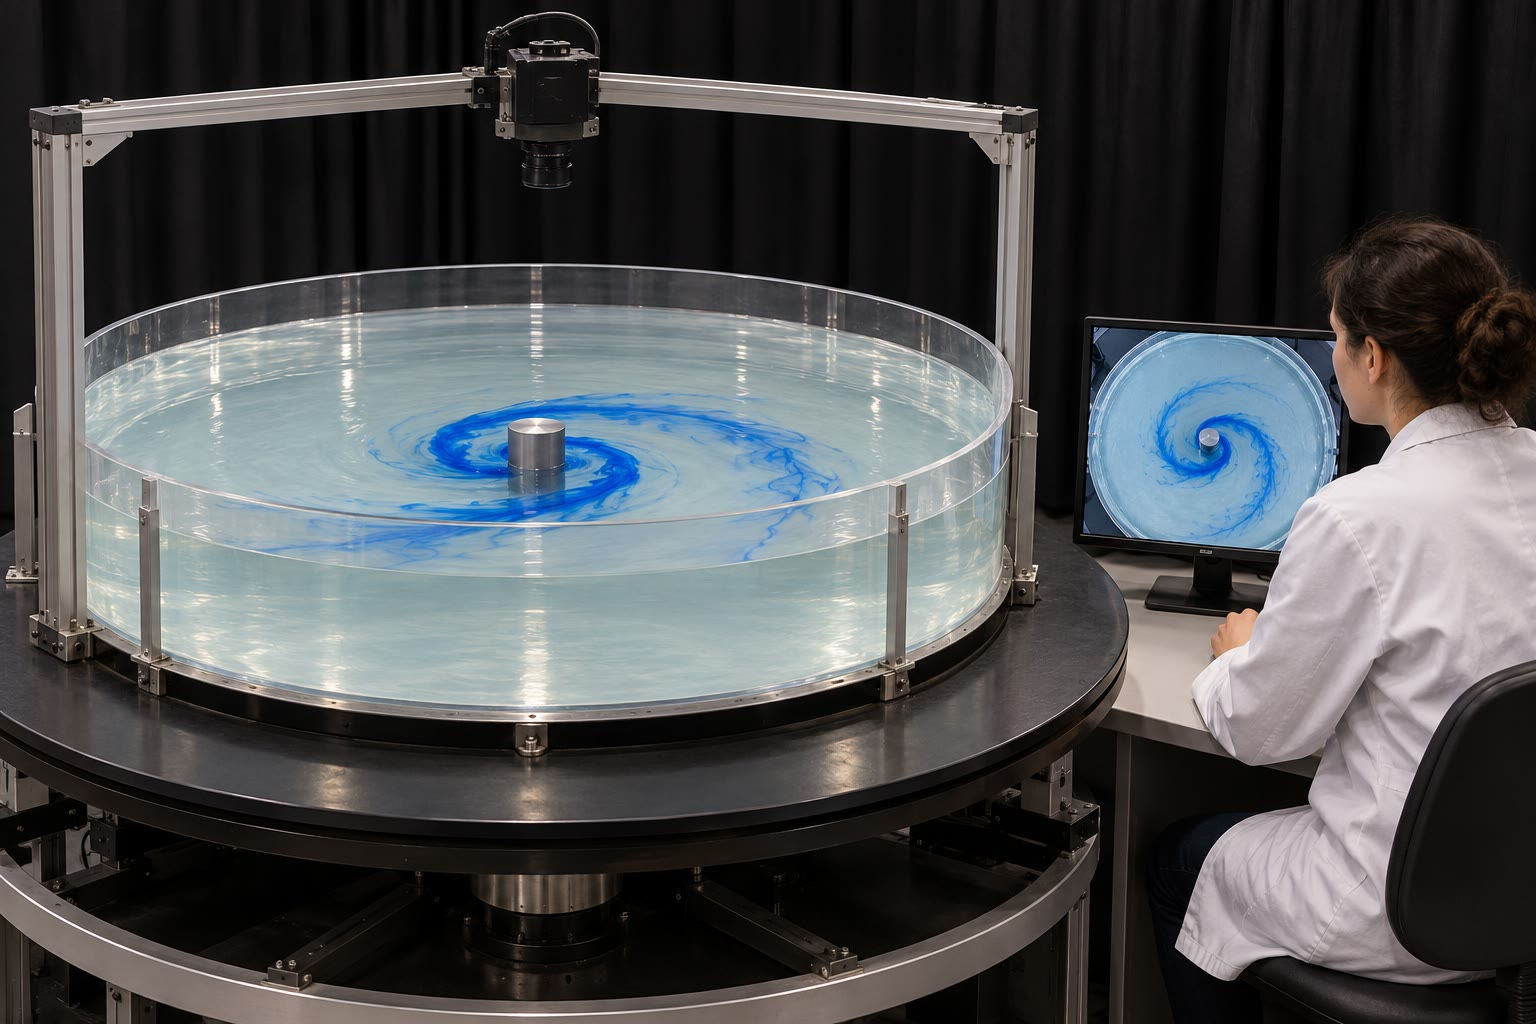
\includegraphics[width=\linewidth]{images/book5/ai/b3-rotating-tank.jpg}

{\scriptsize Bak yang berputar: pewarna berpilin mengelilingi silinder, direkam oleh
kamera yang ikut berputar bersama meja (ilustrasi buatan AI).}
\end{minipage}
\end{inthelab}

\section{Latihan}

\begin{exercise}[$\star$]\label{exo:b3:gfd-foundations:1}
Ambil $\Omega = \qty{7.292115e-5}{rad/s}$. (a)~Hitung parameter Coriolis
dan periode inersia pada \ang{30}, \ang{45} dan \ang{60} LU.
(b)~Hitung jari-jari lingkaran inersia arus
sebesar \qty{0.20}{m/s} pada lintang yang sama. (c)~Bandingkan periode inersia
pada \ang{30} dengan hari sideris, \qty{23.9345}{h}.
\end{exercise}

\begin{exercise}[$\star$]\label{exo:b3:gfd-foundations:2}
Pada \ang{45} LU, hitung \omterm{def:b3:gfd-foundations:numbers}{bilangan Rossby} untuk pusaran debu (\qty{10}{m/s},
\qty{10}{m}), angin laut (\qty{5}{m/s}, \qty{20}{km}), depresi
(\qty{15}{m/s}, \qty{1000}{km}) dan gyre samudra (\qty{0.05}{m/s},
\qty{2000}{km}). Manakah di antara mereka yang mendekati keseimbangan geostrofik?
\end{exercise}

\begin{exercise}[$\star$]\label{exo:b3:gfd-foundations:3}
Pada \ang{45} LU suhu rata-rata troposfer, \qty{250}{K}, turun
ke arah utara sebesar \qty{5}{K} per \qty{1000}{km}. Dengan menggunakan suku pertama
\omterm{thm:b3:gfd-foundations:thermal-wind}{angin termal} terhadap ketinggian, hitung geser vertikal angin barat dan
pertambahan angin sepanjang \qty{10}{km}.
\end{exercise}

\begin{exercise}[$\star$]\label{exo:b3:gfd-foundations:4}
Stabilitas $E = -(1/\rho)\,\mathrm d\rho_\theta/\mathrm dz$ pada kilometer
teratas samudra berada antara \num{50e-8} dan \qty{1000e-8}{m^{-1}};
di palung dalam nilainya \qty{e-8}{m^{-1}}. Hitung $N = \sqrt{gE}$, periode
osilasi daya apung dan $N$ dalam siklus per jam untuk ketiga
nilai tersebut.
\end{exercise}

\begin{exercise}[$\star\star$]\label{exo:b3:gfd-foundations:5}
Suatu sistem cuaca memiliki $U = \qty{10}{m/s}$, $L = \qty{1000}{km}$, $H =
\qty{10}{km}$, pada \ang{45} LU. (a)~Perkirakan kecepatan vertikal dan
percepatan vertikalnya, dan bandingkan yang terakhir dengan $g$ dan dengan
gradien vertikal gangguan tekanan, $fUL/H$. (b)~Hitung
suku Coriolis yang diabaikan $\tilde fu$ dan bandingkan dengan $g$.
\end{exercise}

\begin{exercise}[$\star\star$]\label{exo:b3:gfd-foundations:6}
Ambil $f = \qty{e-4}{s^{-1}}$ dan isobar melingkar berjari-jari
\qty{300}{km}. (a)~Gradien tekanan di sekitar tekanan rendah memberikan $V_g =
\qty{20}{m/s}$: hitung \omterm{def:b3:gfd-foundations:gradient}{angin gradien}. (b)~Di sekitar tekanan tinggi,
$V_g = \qty{5}{m/s}$: hitung \omterm{def:b3:gfd-foundations:gradient}{angin gradien}. (c)~Berapa $V_g$ terbesar
yang mungkin di sekitar tekanan tinggi, dan berapa anginnya saat itu?
\end{exercise}

\begin{exercise}[$\star\star$]\label{exo:b3:gfd-foundations:7}
Sebuah bak berkedalaman \qty{20}{cm} berputar sekali setiap \qty{6}{s}; airnya memiliki $\nu =
\qty{e-6}{m^2/s}$. (a)~Hitung $f = 2\Omega$, lalu \omterm{def:b3:gfd-foundations:numbers}{bilangan Rossby} untuk
aliran \qty{1}{cm/s} yang melewati silinder berdiameter \qty{5}{cm}, serta \omterm{def:b3:gfd-foundations:numbers}{bilangan Ekman}
bak itu. Apakah \omterm{thm:b3:gfd-foundations:taylor-proudman}{kolom Taylor} akan terbentuk? (b)~Teori memberikan
waktu spin-up $H/\sqrt{\nu\Omega}$: hitung dalam menit dan dalam putaran meja.
\end{exercise}

\begin{exercise}[$\star\star$]\label{exo:b3:gfd-foundations:8}
Pada rata-rata zonal Januari 1991--2020, angin barat sebesar \qty{4.27}{m/s}
pada \qty{850}{hPa} dan \qty{40.39}{m/s} pada \qty{250}{hPa} di \ang{30} LU,
\qty{5.99}{m/s} dan \qty{23.17}{m/s} di \ang{45} LU. Dengan $R =
\qty{286.9}{J.kg^{-1}.K^{-1}}$, hitung gradien meridional
suhu rata-rata lapisan pada kedua lintang, dan jelaskan mengapa arus jet lebih kuat
pada \ang{30} LU.
\end{exercise}

\begin{exercise}[$\star\star$]\label{exo:b3:gfd-foundations:9}
(a)~Hitung \omterm{def:b3:gfd-foundations:rossby-radius}{jari-jari deformasi Rossby} troposfer ($N =
\qty{0.0113}{s^{-1}}$, $H = \qty{11}{km}$, \ang{45} LU) dan
samudra bagian atas ($N = \qty{0.00357}{s^{-1}}$, $H = \qty{1000}{m}$, \ang{40.5} LU).
(b)~Dengan $a = \qty{6371}{km}$, hitung $\beta$ pada kedua lintang dan
perubahan relatif parameter Coriolis, $\beta L_R/f$, melintasi setiap jari-jari.
\end{exercise}

\begin{exercise}[$\star\star\star$]\label{exo:b3:gfd-foundations:10}
Sebuah parsel samudra permukaan yang bergerak dengan kecepatan $U$ diperlambat
oleh gesekan linear: $\mathrm du/\mathrm dt = fv - ru$, $\mathrm dv/\mathrm dt = -fu -
rv$. (a)~Selesaikan dengan $w = u + \mathrm iv$ dan jelaskan lintasannya. (b)~Parsel
juga terbawa arus tetap $u_0$ ke timur: berikan
posisinya. (c)~Pada \ang{45} LU dengan $U = \qty{0.2}{m/s}$, $r^{-1} =
\num{4}\text{ hari}$ dan $u_0 = \qty{0.05}{m/s}$, berikan kecepatannya relatif terhadap
arus setelah empat hari dan jarak yang telah dihanyutkannya.
\end{exercise}

\begin{exercise}[$\star\star\star$]\label{exo:b3:gfd-foundations:11}
Melintasi front samudra pada \ang{40} LU, massa jenis air meningkat
ke utara sebesar \qty{1}{kg/m^3} sepanjang \qty{100}{km}, pada lapisan atas
setebal \qty{1000}{m}; di bawahnya, air seragam dan diam. Dengan $\rho_0 =
\qty{1025}{kg/m^3}$, hitung geser vertikal arus dan
arus di permukaan. Ke arah mana arus itu mengalir?
\end{exercise}

\begin{exercise}[$\star\star\star$]\label{exo:b3:gfd-foundations:12}
Kolom rata-rata tahunan pada \ang{40.5} LU, \ang{30.5} BB memiliki
massa jenis potensial $\sigma_\theta = \rho_\theta - \qty{1000}{kg/m^3}$ sebesar 26.029 di
permukaan, 26.697 pada \qty{100}{m}, 27.079 pada \qty{500}{m} dan 27.628 pada
\qty{1000}{m}. (a)~Hitung $N$ pada ketiga lapisan, dalam
\unit{s^{-1}} dan dalam siklus per jam. (b)~Lapisan mana yang paling stabil,
dan mengapa? (c)~Bandingkan nilai-nilainya dengan rentang lapisan atas samudra pada
\cref{exo:b3:gfd-foundations:4}.
\end{exercise}
% ledger: geod5:grs80-defining, earth:Trot, stewart:stability, data:b5-ncep-uwnd, data:b5-woa23-atlantic, earth:Rmean

\section{Soal: Angin di atas Stepa Orrin}

\begin{problem}[{Soal akhir pekan --- rotasi, stratifikasi dan
angin di dataran rekaan pada \ang{48} LU}]
\label{pb:b3:gfd-foundations:1}
Stepa Orrin adalah dataran datar pada \ang{48} LU dengan sebuah danau, Danau Orrin,
lebar \qty{12}{km}, dan sebuah laboratorium kecil dengan tangki berputar. Gunakan
$\Omega = \qty{7.292115e-5}{rad/s}$, $g = \qty{9.81}{m/s^2}$, $R =
\qty{286.9}{J.kg^{-1}.K^{-1}}$ dan $c_p = \qty{1004}{J.kg^{-1}.K^{-1}}$.
Semua nilai stepa, danaunya, dan anginnya adalah rekaan.

\medskip\noindent\textbf{Bagian I --- Apakah rotasi penting?}
\begin{enumerate}
\item Hitung parameter Coriolis dan periode inersia di Orrin.
\item Hitung \omterm{def:b3:gfd-foundations:numbers}{bilangan Rossby} dari lima aliran: air yang mengalir keluar dari bak mandi
  (\qty{0.1}{m/s} sepanjang \qty{0.3}{m}); tangki laboratorium yang berputar
  sekali setiap \qty{10}{s} (dengan $f = 2\Omega_{\text{tangki}}$; \qty{5}{mm/s}
  sepanjang \qty{0.2}{m}); angin sore dari danau (\qty{5}{m/s},
  \qty{20}{km}); sebuah depresi (\qty{15}{m/s}, \qty{1000}{km}); gyre dari sebuah
  cekungan samudra pada lintang yang sama (\qty{0.05}{m/s}, \qty{2000}{km}).
\item Manakah dari aliran ini yang merasakan rotasi yang menggerakkannya, dan mana yang
  mendekati geostrofik?
\item Hitung \omterm{def:b3:gfd-foundations:numbers}{bilangan Ekman} untuk tangki (kedalaman \qty{0.2}{m}, $\nu =
  \qty{e-6}{m^2/s}$), depresi (viskositas eddy \qty{10}{m^2/s},
  kedalaman \qty{10}{km}), dan gyre (viskositas eddy \qty{e-3}{m^2/s},
  kedalaman \qty{1000}{m}).
\item Lapisan Ekman memiliki ketebalan $\delta = \sqrt{2\nu/f}$. Tunjukkan bahwa
  $\delta/H = \sqrt{2\,\mathrm{Ek}}$ dan hitung $\delta$ untuk tangki dan untuk
  udara di stepa.
\item Apa yang dikatakan bilangan-bilangan ini tentang tempat gesekan berpengaruh?
\end{enumerate}

\medskip\noindent\textbf{Bagian II --- Angin di permukaan tanah.}
\begin{enumerate}[resume]
\item Di permukaan tanah, tekanannya \qty{1012.9}{hPa} dan suhunya
  \qty{288.1}{K}. Hitung massa jenis udara.
\item Tekanan permukaan laut turun ke utara sebesar \qty{4}{hPa} per
  \qty{300}{km}. Hitung angin geostrofik dan berikan arahnya.
\item Gradien yang sama mengelilingi sebuah depresi yang isobarnya memiliki jari-jari
  \qty{600}{km}. Hitung \omterm{def:b3:gfd-foundations:numbers}{bilangan Rossby} dari isobar dan
  \omterm{def:b3:gfd-foundations:gradient}{angin gradien}.
\item Gradien yang sama mengelilingi sebuah antisiklon dengan jari-jari yang sama.
  Hitung \omterm{def:b3:gfd-foundations:gradient}{angin gradien} dan gradien tekanan terbesar, dalam
  \unit{hPa} per \qty{300}{km}, yang masih dapat dipertahankan antisiklon ini.
\end{enumerate}

\medskip\noindent\textbf{Bagian III --- Stratifikasi.}
\begin{enumerate}[resume]
\item Suhu troposfer turun sebesar \qty{6.49}{K/km}.
  Hitung laju penurunan adiabatik kering $g/c_p$, dan $N$ serta periode
  osilasi daya apung pada \qty{5}{km}, dengan suhu
  \qty{255.7}{K}.
\item Di atas \qty{11}{km} udara bersifat isotermal pada \qty{216.6}{K}. Tunjukkan bahwa
  $N^2 = g^2/(c_pT)$ di sana, dan hitung $N$ serta rasionya terhadap nilai
  pada pertanyaan~11.
\item Hitung \omterm{def:b3:gfd-foundations:rossby-radius}{jari-jari deformasi Rossby} troposfer Orrin, dengan $N$ dari
  pertanyaan~11 dan $H = \qty{10}{km}$, lalu bandingkan dengan ukuran
  depresi pada Bagian~I.
\item Pada musim panas, \qty{20}{m} lapisan atas Danau Orrin lebih ringan daripada
  air dalam sebesar \qty{1.5}{kg/m^3} ($\rho_0 = \qty{1000}{kg/m^3}$). Hitung
  gravitasi tereduksi $g' = g\,\Delta\rho/\rho_0$, kecepatan $\sqrt{g'h}$ dari
  gelombang internal lambat pada lapisan atas, dan \omterm{def:b3:gfd-foundations:rossby-radius}{jari-jari deformasi Rossby}
  $\sqrt{g'h}/f$.
\item Apakah rotasi Bumi akan membentuk gerakan internal danau?
\end{enumerate}

\medskip\noindent\textbf{Bagian IV --- Angin termal.}
\begin{enumerate}[resume]
\item Dua stasiun radiosonde berjarak \qty{600}{km} pada
  meridian yang sama. Suhu rata-rata lapisan dari permukaan tanah,
  \qty{1013}{hPa} hingga \qty{265}{hPa}, sekitar \qty{10}{km}, adalah \qty{253.0}{K}
  di stasiun selatan dan \qty{249.4}{K} di stasiun utara. Hitung
  gradien suhu meridional dalam \unit{K} per \qty{1000}{km}.
\item Ketebalan lapisan di antara dua tekanan adalah $\Delta z = (R\bar
  T/g)\ln(p_b/p_t)$. Hitung di kedua stasiun, dan kemiringan permukaan
  \qty{265}{hPa} relatif terhadap permukaan tanah.
\item Turunkan kenaikan angin geostrofik dari permukaan tanah hingga
  \qty{265}{hPa}, dari kemiringan itu.
\item Hitung kenaikan yang sama dengan teorema \omterm{thm:b3:gfd-foundations:thermal-wind}{angin termal} dalam koordinat tekanan.
\item Apakah udara di stepa \omterm{def:b3:gfd-foundations:baroclinic}{barotropik} atau \omterm{def:b3:gfd-foundations:baroclinic}{baroklinik}? Berapa angin
  pada \qty{265}{hPa} seandainya udara itu \omterm{def:b3:gfd-foundations:baroclinic}{barotropik}?
\item Hitung kenaikan dari suku pertama \omterm{thm:b3:gfd-foundations:thermal-wind}{angin termal} dalam
  ketinggian, dengan suhu rata-rata troposfer standar antara 0
  dan \qty{10}{km}, \qty{255.7}{K}, dan bandingkan.
\item Hitung angin pada \qty{541}{hPa}, sekitar \qty{5}{km}, dengan menganggap bahwa
  gradien suhu sama di setiap aras.
\item Bilangan Richardson $N^2/(\partial u/\partial z)^2$ harus turun di bawah
  0.25 agar geser memicu turbulensi. Hitung untuk troposfer
  Orrin.
\item Pada Januari, angin barat rata-rata zonal pada \qty{250}{hPa} adalah \qty{23.2}{m/s}
  di \ang{45} LU dan \qty{40.4}{m/s} di \ang{30} LU. Bandingkan dengan angin di
  Orrin, dan jelaskan mengapa angin lokal dapat melampaui rata-rata zonal.
\item Berikan angin geostrofik pada \qty{10}{km} di atas Stepa Orrin.
\end{enumerate}
\end{problem}
% ledger: geod5:grs80-defining, stewart:stability, data:b5-ncep-uwnd, nasa:grc-atmos
